% !TeX root = ../main.tex

% Implementation
% Explain all low-level implementation level details
\chapter{Implementation}\label{chapter:implementation}
In this chapter, we will go over low-level implementation details and explain what we had to do in order to get the reproducer working.
Firstly we will talk about our additions to the verifier.
Then we will talk about our Python program and explain the functionality of the two classes we have designed.
Finally, we will go over the cases where the verifier might not work as expected.

\section{Additions to the Focaccia}
Focaccia is a full-fledged verifier that can be used to find bugs in emulators that stem from the wrong implementation of instructions.
But because it was designed as a verifier it lacks some useful features that would be of help to the reproducer.

Firstly the original verifier would not return the actual state of the program before the execution of an instruction.
This of course made it quite difficult to know what was inside the memory and registers.
We patched the verifier to return the snapshot of the program.

Our second addition was to the symbolic execution part of the verifier.
The symbolic expressions that the verifier can isolate are quite helpful.
It can return the following values from a given symbolic expression:
\begin{itemize}
    \item Symbolic expressions of the used and changed memory addresses
    \item A list of used registers
\end{itemize}
Both of these results are quite helpful since we can know which registers need to be restored and which memory locations need to have which values.
If we could change anything without considering the underlying hardware mechanisms like paging, permissions, and the actual location of the program in the memory, this might have been enough.
However since this is not possible in the scope of this project, we had decided to allocate space on the data section and use it for memory.
This meant we needed to find the registers that were specifically used for addressing the memory and change the values of these registers to point to the addresses in the data section.

We made this by adding a function to the symbolic execution program, which would evaluate any given expression except a register.
This meant that given a symbolic expression that points to an address, we could extract the used registers.
Then we can be sure that these registers are for addressing memory and handle them as such.

The same mechanism also works for the stack.
We filter the symbolic expressions that point to memory for the stack pointer, thereby assessing them for whether they were used in the stack.

\section{Python Classes}
Our reproducer was implemented in the Python programming language and is made up of two classes.
The first one which is target agnostic is called ReproducerEntry.
This class is used to extract information from the snapshot and the symbolic expressions.
The second class is called x86Reproducer.
As the name suggests this class is x86 architecture-specific and it is tasked with producing assembly instructions for its architecture.
The flow of data can be seen in figure \ref{fig:rep_ent}.
As the figure suggests ReproducerEntry splits the snapshot using the symbolic expression and sets the x86Reproducer with the necessary values.
After which the x86Reproducer prints the assembly code.

\begin{figure}[ht]
    \centering
    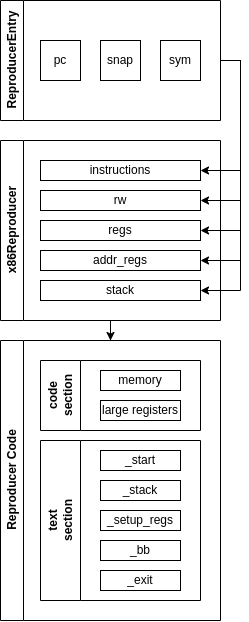
\includegraphics[width=0.5\linewidth]{figures/rep_ent}
    \caption{Flow of the reproducer including the ReproducerEntry and x86Reproducer classes.}
    \label{fig:rep_ent}
\end{figure}

\subsection{ReproducerEntry}
The backbone of our reproducer is the ReproducerEntry class.
It lets us find all of the necessary data using the snapshot and the symbolic expressions.
The main functionality of this class is shown in figure \ref{fig:rep_ent}, but we will go over the details:

\begin{itemize}
    \item get\_instructions:
    This function returns a list of instructions that make up the erroneous basic block.
    These instructions are received from only the symbolic expression.
    \item get\_rw\_addr:
    This function returns a dictionary of reads that will happen during the execution of the basic block and the writes that will happen as a result.
    Each entry is for a single byte and its key is the address.
    The reads keep the original values while writes are initialized with zeros.
    \item get\_regs:
    This function returns the dictionary of registers that are needed for the execution of the basic block.
    \item get\_addr\_regs:
    This function also returns a dictionary of registers.
    However, these are dictionaries that were only used for addressing memory.
    And the values of these dictionaries are not the register's values but the actual address that they were used to address.
    \item get\_stack:
    This function returns two values.
    Firstly it returns the number of bytes that were subtracted from the stack pointer (either due to push operations or just subtraction from the stack pointer).
    Secondly, it returns the values that were in the stack.
    If a particular value was not used, then its place is filled with zeros.
\end{itemize}

As we have shown the ReproducerEntry is a versatile class that can be used to extract everything that we need from the snapshot and the symbolic expression.

\subsection{x86Reproducer}
This class is the part that produces the assembly instructions.
It is specifically designed to produce x86 assembly.
It receives all the information from the ReproducerEntry and doesn't directly use the snapshot or the symbolic expression.

In the data section, we use the register dictionary and the read/write dictionary to initialize the values.
In the text section, the basic block is combined with stack and register setup code along with start and exit stubs.
The stack setup only uses what was returned from the stack values, while the register setup uses both the regular register dictionary and the addresses register dictionary.

\section{Shortcomings}
When trying to understand the shortcomings of the reproducer it is important to keep in mind that it was designed as an add-on to the verifier, which in turn depends on Miasm to work properly.
As we have mentioned before our reproducer does have some shortcomings regarding special registers and some instructions.
In this section, we will go over these cases and try to explain why they are difficult to deal with.

When thinking about why it is not possible to perfectly replicate bugs, there are two very important points to consider.
First of all computer programs run step by step.
Each step changes the state of the program, values are written to the memory, and registers are changed.
However, this is not all of the changes.
When a program is running stack frames are built or destroyed, new pages are added, permissions are updated, and data that is handled by the kernel is changed.

A program is more than just its address space, when trying to understand bugs that stem from emulation we need to keep in mind that the hardware in the background is also a part of the program.
To perfectly replicate the state, all of the aforementioned data needs to be changed.
However this is not possible, there is no mechanism to replicate all of these except to run the exact program until that point.
This means the best we can do is approximate the state that causes the bugs.

The second point is the symbolic expressions.
They are quite good at showing state transitions and building a tree for the execution path.
But they are an abstraction and therefore lack details that might be contributing to the bugs.
They do show what instructions do but they are all on a transactional level.
For example, a symbolic expression might show a read operation, but it doesn't necessarily show whether the read address was an IO port or it was on a page that didn't exist.
Therefore we use it to guide us the best we can.

\subsection{Shortcomings of the Reproducer}
The reproducer has managed to reproduce bugs and code snippets that generally use simpler instructions that do calculations, however, it still has some shortcomings regarding more complicated instructions that affect the program flow or some registers that are used for controlling the hardware.

\subsubsection{Instruction Pointer}
In CPUs, the instruction pointer is used to select the next instruction which will be executed.
Normally each instruction increments it by that instruction size.
However, there are some instructions like jump, call, and return that change the instruction pointer arbitrarily.
In these cases, the execution path also changes to a different location.

Most emulators and binary translators work either on an instruction basis or a basic block basis.
In both cases, only the last instruction can be one of the aforementioned instructions.
Since we can just ignore that last instruction and still get the same calculation, we have chosen to ignore it.
This way we can keep the verifier simpler.

\subsubsection{Segment Registers}
These registers were designed to let the original x86 CPU address more than 64 KB of memory.
However, these are currently used for other purposes like thread-local storage and canary-based stack protection.
We have left out these registers because changing them is quite likely to cause any program to crash.

\subsubsection{Return Address}
When we are building the stack for the erroneous basic block, we set the stack by using the values directly from the original snapshot.
And we push these values directly after the start section.
However, this means that the return address of the function is wrong.
It is either zero, if it is not used at all, or it is the original return address.
Both of these values are likely to crash the program if used for returning from the start section but since we directly use the exit syscall it should not have any effect on the program.

\subsubsection{Indirect Memory Access}
Although our program can find memory access by using reads and writes, we only look for them in the registers.
This makes sense since to address a memory location we need to use at least one register.
However in cases where a memory location has a pointer to a different address our program cannot recognize them and it will copy the same value, meaning it would be pointing to an unknown location.

This cannot happen on a single instruction since the address needs to be already in the register.
In case a basic block is used and this problem arises, the best way to deal with it would be to run the reproducer on a single instruction basis.
This method should prevent programs from indirect memory access in a single basic block. 

\subsection{Segmentation Faults}
As we have mentioned previously we cannot replicate \ac{segfault}s even though we have all the necessary information because without the state that happens after the \ac{segfault} the verifier cannot notice them.
This weakness can be solved by adding a \ac{segfault} error to the verifier that happens when the emulator log is shorter than expected.
In that case, the reproducer can theoretically produce a program that can trigger the same \ac{segfault}.

However, this is not as simple as it sounds.
This might not always work because some \ac{segfault}s happen on special cases like alignment of the data or permissions of the memory section.
Unfortunately, the reproducer is oblivious to these things and therefore it is difficult to replicate them.

\subsection{Shortcomings of the Symbolic Execution Engine}
We have decided to add this section here to mention that our project relies on the verifier to function which in turn relies on the symbolic execution engine.
This means if the symbolic execution engine has any problems like unimplemented instructions our reproducer also suffers from it.

We have tested our reproducer with many different programs and we came to notice that most instructions that should have caused the bugs were not implemented in Miasm.
This had multiple different effects on the reproducer.
Sometimes instructions would be translated wrongly and sometimes they would be missing.
This has no simple solution except to fix Miasm itself.
